\documentclass[11pt,twoside,a4paper,final]{llncs}
\usepackage[utf8]{inputenc}
\usepackage[T1]{fontenc}
\usepackage[MeX]{polski}
\usepackage{graphicx}
\usepackage{url}
\usepackage{hyperref}
\bibliographystyle{splncs}

\begin{document}

\date{21 stycznia 2013}
\title{Przegląd dziedziny bibliotek i narzędzi do tworzenia wykresów}

\author{Łukasz Szewczyk}
\institute{Politechnika Warszawska, Wydział Elektroniki i Technik Informacyjnych}
\maketitle


\section{Wstęp}
Przegląd ten zawiera opis kilku wybranych bibliotek służących do tworzenia wykresów. Zostały tu opisane zarówno biblioteki przeznaczone dla Qt i C++, jak i innych technologii i języków. Ponadto uwzględniono rozwiązania darmowe oraz komercyjne.

\section{Biblioteki Qt} 
\subsection{Qwt}
\textit{Qt Widgets for Technical Applications} to otwarta biblioteka służąca głównie do tworzenia  wykresów technicznych. Jak sama nazwa wskazuje, biblioteka ta udostępnia programistom gotowe widgety, więc niezbyt nadaje się do prezentowania danych w aplikacjach napisanych w Qt~Quick. Największymi zaletami \textit{Qwt} są jej duże możliwości oraz wsparcie społeczności. \textit{Qwt} jako jedna z~nielicznych umożliwia tworzenie wykresów z osią logarytmiczną. Biblioteka zawiera szerokie API służące do przeprowadzania różnorakich operacji na wykresach, m.in. skalowania, powiększania i zaznaczania. Wadą jest wygląd wykresów, które wyglądają jak oscylogramy, przykład na rys. \ref{rys:wykres:sinus}. Poza wykresami, biblioteka ta udostępnia również inne widgety, takie jak suwaki czy pokrętła typowe dla elektronicznych urządzań pomiarowych.
\begin{figure}
\centering
\caption{Przykładowy wykres Qwt}\label{rys:wykres:sinus}
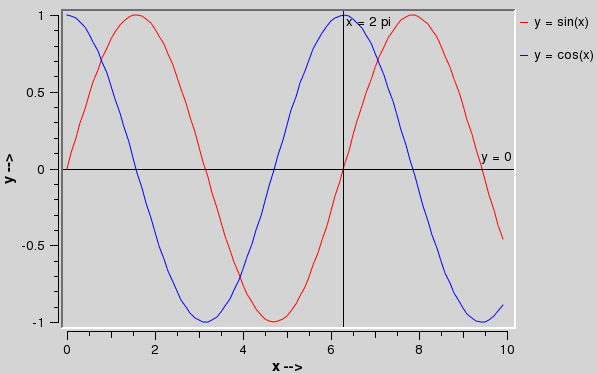
\includegraphics[scale=0.4]{sinus.png}
\end{figure}

\subsection{Qt Commercial Charts}
Jest to komercyjna biblioteka stworzona przez właściciela Qt -- firmę Digia. Nastawiona jest głównie na tworzenie wykresów biurowych i udostepnia chyba wszystkie popularne wykresy tego typu. Pozwala ona na całkiem sporą interakcję użytkownika z wykresami, m.in. przybliżanie fragmentów wykresów, wyświetlanie dymków uszczegóławiających dane wykresu. Ponadto wykresy tworzone za pomocą \textit{Charts} wyglądają dobrze pod względem estetycznym, ich styl (czcionka i~tonacje kolorów) może być zmieniany za pomocą mechanizmu motywów, a~animacja procesu budowania wykresów nadaje prezentacji danych atrakcyjnej dynamiki. Biblioteka umożliwia wyswietlania wykresów różnego typu w~jednym układzie współrzędnych, obsługę osi logarytmicznej oraz tworznie osi nie tylko liczbowych, ale także czasu czy daty. Ważną cechą biblioteki jest wsparcie dla Qt~Quick.

\subsection{GobChartWidget}
Jest to projekt rozwijany przez osobę, bądź grupę programistów o nazwie Goblin. Jest to biblioteka open source-owa, a~jej źródła są dostępne na stronie twórcy. Udostępnia ona jedynie wykresy słupkowe, liniowe i~kołowe, a~ich wygląd jest dużo słabszy od tych udostępnianych przez Digię. Ciekawą własnością jest fakt, że źródłem danych dla wykresu musi tutaj być model z architektury \textit{Model-Widok-Delegat} bądź plik XML o~odpowiedniej strukturze.


\section{Biblioteki i narzędzia dla innych technologii}
\subsection{JFreeChart}
Darmowa i najpopularniejsza wg. \url{http://stackoverflow.com} biblioteka do tworzenia wykresów w języku Java. Z popularnych wykresów biurowych, nie udostępnia jedynie warstwowego. Nie można przyczepić się do wykresów pod względem wyglądu, ale też nie wyróżniają się one niczym pozytywnym na tle konkurencji. Na duży plus zasługuje możliwość dodawania animacji przy budowaniu wykresu.

\subsection{CairoPlot}
Jest to darmowa biblioteka dla języka Python, która ma całkiem szeroki repertuar wykresów, oferuje m.in. wykres Gantta. Wszystkie z nich wyglądają bardzo estetycznie, a chyba najlepiej prezentuje się wykres słupkowy, który został umieszczony w logo \textit{CairoPlot} na rys. \ref{rys:logo:cairo}. Kolejnym elementem podnoszącym wartość estetyczną tych wykresów jest system motywów. Tworzenie nowych wykresów jest banalnie proste i wymaga podania odpowiednich parametrów do jednej funkcji.

\begin{figure}
\centering
\caption{Logo biblioteki CairoPlot}\label{rys:logo:cairo}
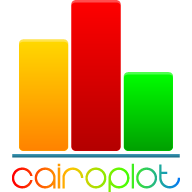
\includegraphics[scale=0.6]{cairo_plot.png}
\end{figure}

\subsection{Google Chart Tools}
Jest to zbiór narzędzi do umieszczania wykresów na witrynach internetowych. Zapewnia zdecydowanie najszerszy zakres wykresów. Od podstawowych, jak liniowy czy kołowy, po tak wymyślne diagramy jak \textit{Geochart}, czyli wykres przedstawiający dane w kontekście terytoriów państw czy kontynentów.
Wykresy prezentują się bardzo dobrze, nawet wykres liniowy nie jest tu ,,kanciasty''. Zapewniona jest również duża interakcyjność wykresów. Wszystkie elementy reagują na ruchy myszki, a po najechaniu na elementy reprezentujące dane, pojawiają się podpowiedzi. Zmiana wartości dla danej próbki danych może być animowana, tak samo jak proces budowy całego wykresu. Znajdziemy tu rozbudowane API służące podłączaniu różnych źródeł danych, np. baza danych.

\subsection{MS Office}
Najpopularniejszy pakiet biurowy, dzieło firmy Microsoft. Zarówno w arkuszach kalkulacyjnych jak i prezentacjach tworzonych w tym pakiecie bardzo często pojawiają się wykresy, których wybór jest bardzo duży.
Dane tutaj są albo wklepywane ręcznie, np. dla wykresu w prezentacji PowerPoint, albo pobierane z tabelki Excela. 

\section{Dostępne typy wykresów}
\subsection{Qt}
\begin{tabular}{|c|c|c|c|}
\hline
&  Qwt & Commercial Charts & GobChart\\
\hline
Bąbelkowy & N & T & N\\
\hline
Kołowy & N & T & T\\
\hline
Liniowy & T & T & T\\
\hline
Pierścieniowy & N & T & N\\
\hline
Słupkowy & N & T & T\\
\hline
Warstwowy & N & T & N\\
\hline
XY (punktowy) & T & T & N\\
\hline
\end{tabular}

\subsection{Pozostałe}
\begin{tabular}{|c|c|c|c|c|}
\hline
& JFreeChart & CairoPlot & Google & MS Office\\
\hline
Bąbelkowy & T & N & T & T\\
\hline
Gantta & T & T & N & N\\
\hline
Geomap & N & N & T & N\\
\hline
Kołowy & T & T & T & T\\
\hline
Liniowy & T & T & T & T\\
\hline
Pierścieniowy & T & T & N & T\\
\hline
Słupkowy & T & T & T & T\\
\hline
Warstwowy & T & N & N & T\\
\hline
XY (punktowy) & T & N & T & T\\
\hline
\end{tabular}

\section{Elementy wspólne}
Analizując powyższe biblioteki dochodzimy do wniosku, że można wykroić z nich część wspólną, stanowiącą podstawową funkcjonalność niezbędną dla biblioteki tego typu. Te cechy wspólne to:
\begin{itemize}
\item{podstawowe wykresy, takie jak liniowy, słupkowy i kołowy,}
\item{elementy dekoracyjne, takie jak osie, siatka i legenda,}
\item{interakcja, polegająca na zaznaczaniu i przybliżaniu fragmentów wykresów,}
\item{interfejs do danych -- każda z bibliotek wprowadza jakiś ujednolicony sposób komunikacji wykresu z modelem zawierającym dane,}
\item{efekty 3D, mniej lub bardziej udane próbu nadania wykresom głębi.}
\end{itemize}

\section{Elementy unikalne}
Prawie każda biblioteka zawiera wartościowe elementy niepowtarzalne lub rzadko spotykane:
\begin{itemize}
\item{animacja towarzysząca tworzeniu wykresów oraz ich przebudowywaniu,}
\item{motywy pozwalające na tworzenie wykresów w~różnych, jednolitych stylach,}
\item{rozszerzenie interaktywności wykresu poprzez podpowiedzi do próbek danych lub ruchome wykresy (np. niezależne obracanie pierścieni wykresu pierścieniowego),}
\item{plik XML lub CSV jako źródło danych,}
\item{tworzenie wykresów w formacie SVG.}
\end{itemize}

\section{Wnioski}
Jak widać istnieje trzon funkcjonalności, który po prostu trzeba napisać, aby tworzona biblioteka miała sens. Pozostałe elementy stanowią ciekawe dodateki, który mogą być dodawane w kolejnych iteracjach. W dalszej fazie pracowni warto zwrócić szczególną uwagę na uniwersalność biblioteki, tak aby nie stworzyć narzędzia tak mało elastycznego jak \textit{GobChartWidget}. Jeśli chodzi o funkcjonalność, warto wzorować się na rozwiązaniach firm Digia oraz Google.

\end{document}
